
    \documentclass{lebook}
    \usepackage{lelists}
    \setlength{\listtopsep}{0pt}
    \setlength{\leftlistindent}{0pt}
    \setlength{\rightlistindent}{0pt}

    \usepackage{lefonts}
    \usepackage{lecode}
    \usepackage{legraphicextensions}
    \graphicspath{{Figures/}}

    \usepackage{lesubscripts}
    \usepackage[pdfauthor={Lance A. Endres}, pdftitle={WinEdt Installation Notes, colorlinks}]{lehyperlink}
    \usepackage{leheadersandfooters}

    \usepackage{leaddress}

    \usepackage{times}

    \newcommand{\tbs}{$\backslash$}

	%%%%%%%%%%%%%%%%%%%%%%%%%%%%%%%%%%%%%%%%%%%%%%%%%%%%%%%%%%%%%%%%%%%%%
	% BEGIN DOCUMENT
	%%%%%%%%%%%%%%%%%%%%%%%%%%%%%%%%%%%%%%%%%%%%%%%%%%%%%%%%%%%%%%%%%%%%%

	\pagestyle{leplainheader}
	\begin{document}

    \chapter{Additional Information}
See the following directory for additional installation requirements.
    \begin{plainlist}
        \item \codetext{C:\tbs{}Custom Program Files\tbs{}LaTeX\tbs{}Processing Support\tbs{}Notes\tbs{}}
    \end{plainlist}



    \chapter{WinEdt v9 and Below}
    \section{Adding a Custom Button}

    \begin{numberedlist}
        \item Open: \codetext{Options$\rightarrow{}$Preferences$\rightarrow{}$Advanced}

        \item Edit the \codetext{WinEdt.btn} file as shown in \figurename~\ref{fig:addcustombutton}.

        \item Add a line to the end of the file similar to:
            \begin{plainlist}
                \item \codetext{204 \%B\tbs{}Bitmaps\tbs{}Buttons\tbs{}Command Prompt.bmp}
                \item \codetext{205 \%B\tbs{}Bitmaps\tbs{}Buttons\tbs{}Recycle.bmp}
                \item \codetext{206 \%B\tbs{}Bitmaps\tbs{}Buttons\tbs{}Recycle.bmp}
                \item \codetext{207 \%B\tbs{}Bitmaps\tbs{}Buttons\tbs{}image.bmp}
            \end{plainlist}
    \end{numberedlist}
The number in that line will be the button number is the toolbar setup.
Use a bmp from one previously defined.
    \begin{figure}
      \centering
      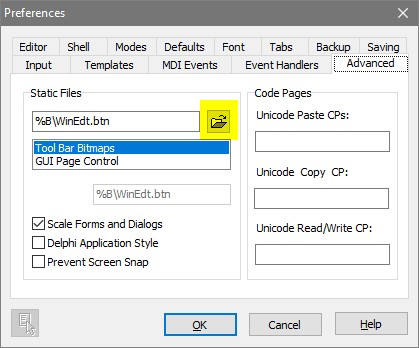
\includegraphics[width=3in]{addcustombutton}
      \caption{Edit the \codetext{WinEdt.btn}}
      \label{fig:addcustombutton}
    \end{figure}



    \section{Add a New Command}
Enter the menu setup as shown in \figurename~\ref{fig:entermenusetup}.
    \begin{figure}
        \centering
        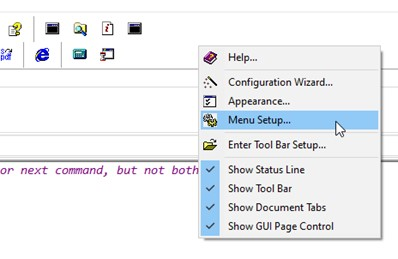
\includegraphics[width=3in]{entermenusetup}
        \caption{Enter menu setup.}
        \label{fig:entermenusetup}
    \end{figure}

Double click an entry (as shown in \figurename~\ref{fig:doubleclickmenuitemtoopen} to open it for editing.
    \begin{figure}
        \centering
        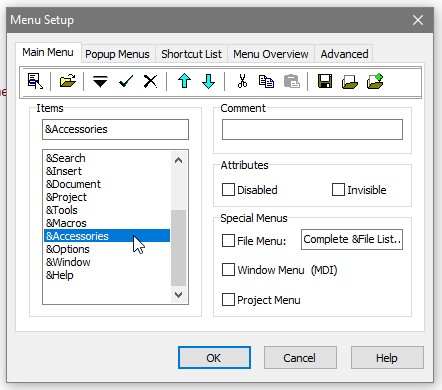
\includegraphics[width=3in]{doubleclickmenuitemtoopen}
        \caption{Double click the menu item to open the editor for it.}
        \label{fig:doubleclickmenuitemtoopen}
    \end{figure}

Setup all the highlighted sections in \figurename~\ref{fig:commandsetup}.  The commands to use are below.
    \begin{plainlist}
        \item Make Document
        \begin{plainlist}
            \item Macro:    \codetext{Run('run\_make\_document.bat "\%N"','',0,0,'Make Document',1,1);}
            \item Start in: \codetext{\%P}
        \end{plainlist}
        \item Clean Temp Files
        \begin{plainlist}
            \item Macro:    \codetext{Run('clean\_temp\_files.bat','',0,0,'Clean Up',1,1);}
            \item Start in: \codetext{\%P}
        \end{plainlist}
        \item Clean All Output
        \begin{plainlist}
            \item Macro:    \codetext{Run('clean\_all\_output.bat','',0,0,'Clean Up',1,1);}
            \item Start in: \codetext{\%P}
        \end{plainlist}
        \item Convert All Images
        \begin{plainlist}
            \item Macro:    \codetext{Run('convert\_all\_images.bat','',0,0,'Make Images',1,1);}
            \item Start in: \codetext{\%P\tbs{}Figures\tbs{}Image Sources\tbs{}}
        \end{plainlist}
    \end{plainlist}

    \begin{figure}
        \centering
        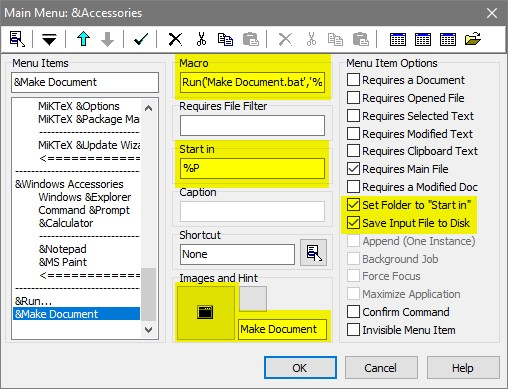
\includegraphics[width=3in]{commandsetup}
        \caption{Ensure all the highlighted sections are set correctly.}
        \label{fig:commandsetup}
    \end{figure}


    \chapter{WinEdt v10 and Above}
    \section{Options Interface}
In version 10 and above the procedure has changed.  Every thing is accessed through the \textit{Options Interface}.  Right click on the toolbar and select the button for it (see \figurename~\ref{fig:openingoptionsinterface}).  The \textit{Options Interface} is shown in \figurename~\ref{fig:optionsinterface}.
    \begin{figure}
		\centering
		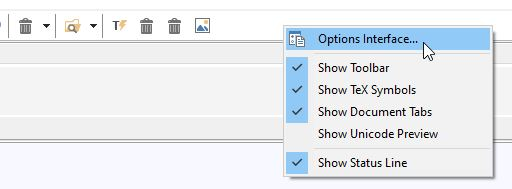
\includegraphics[width=3.25in]{openingoptionsinterface}
		\caption{Opening the \textit{Options Interface} panel.}
		\label{fig:openingoptionsinterface}
    \end{figure}

    \begin{figure}
		\centering
		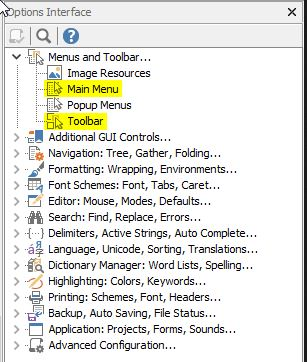
\includegraphics[width=2.25in]{optionsinterface}
		\caption{The \textit{Options Interface} panel.}
		\label{fig:optionsinterface}
    \end{figure}


	\section{Add Menu Items}
	\begin{numberedlist}
		\item Open the \textit{Main Menu} document from the \textit{Options Interface} panel.
		\item Search for \codetext{"TeX\_Menu"}.
		\item Under it, add the following:
	\end{numberedlist}
	\begin{plainlist}
		\item \codetext{ITEM="Make\_Document"}
		\begin{plainlist}
			\item \codetext{CAPTION="Make Document"}
			\item \codetext{IMAGE="TeXTeXif"}
			\item \codetext{SAVE\_INPUT=1}
			\item \codetext{MACRO="Run('\%P\tbs{}run\_make\_document.bat ""\%N""','\%P',0,0,'Make Document',1,1);"}
			\item \codetext{REQ\_FILTER=:"\%!M=TeX"|"\%!M=TeX:STY"|"\%!M=TeX:AUX"}
		\end{plainlist}
		\item \codetext{ITEM="Clean\_Temp\_Files"}
		\begin{plainlist}
			\item \codetext{CAPTION="Delete Temporary Files"}
			\item \codetext{IMAGE="Recycle"}
			\item \codetext{SAVE\_INPUT=1}
			\item \codetext{MACRO="Run('clean\_temp\_files.bat','\%P',0,0,'Clean Temp Files',1,1);"}
		\end{plainlist}
		\item \codetext{ITEM="Clean\_All\_Output"}
		\begin{plainlist}
			\item \codetext{CAPTION="Delete All Output Files"}
			\item \codetext{IMAGE="Recycle"}
			\item \codetext{SAVE\_INPUT=1}
			\item \codetext{MACRO="Run('clean\_all\_output.bat','\%P',0,0,'Clean All Output Files',1,1);"}
		\end{plainlist}
		\item \codetext{ITEM="Convert\_All\_Images"}
		\begin{plainlist}
			\item \codetext{CAPTION="Convert All Images"}
			\item \codetext{IMAGE="Image"}
			\item \codetext{SAVE\_INPUT=1}
			\item \codetext{MACRO="Run('convert\_all\_images.bat','\%P\tbs{}Figures\tbs{}Image Sources',0,0,'Convert All Images',1,1);"}
		\end{plainlist}
	\end{plainlist}

	\section{Add Toolbar Buttons}
	\subsection{Add \textit{Save All}}
Right click on toolbar
Find the line:
	\begin{plainlist}
		\item \codetext{BUTTON="Save"}
	\end{plainlist}

and just below it add:
	\begin{plainlist}
		\item \codetext{BUTTON="Save\_All"}
	\end{plainlist}

	\subsection{Custom Processing Buttons}
Go to the end of the main toolbar entry and add the following lines:
	\begin{plainlist}
		\item \codetext{BUTTON="|"}
		\item \codetext{BUTTON="Make\_Document"}
		\item \codetext{BUTTON="Clean\_Temp\_Files"}
		\item \codetext{BUTTON="Clean\_All\_Output"}
		\item \codetext{BUTTON="Convert\_All\_Images"}
	\end{plainlist}

	\subsection{Templates}
Open the file:
\codetext{\%b\tbs{}Templates\tbs{}LaTeX\tbs{}Figure.ltx}
E.g.:
\codetext{C:\tbs{}Users\tbs{}lance.endres\tbs{}WinEdt Team\tbs{}WinEdt 11\tbs{}Templates\LaTeX\tbs{}Figure.ltx}

and replace its contents with the one found in the file:
\codetext{C:\tbs{}Custom Program Files\tbs{}WinEdt\tbs{}src V10 and Above}

	\subsection{Running Multiple Instances}
	\begin{numberedlist}
		\item Select the \codetext{Additional Preferences} section of the \codetext{Application: ...} as shown in \figurename~\ref{fig:additionalpreferences}.
		\item Change the line \codetext{RUN\_ONE\_INSTANCE\_ONLY=1} to \codetext{RUN\_ONE\_INSTANCE\_ONLY=0}.
	\end{numberedlist}
	\begin{figure}
		\centering
		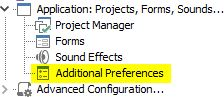
\includegraphics[width=2.5in]{additionalpreferences}
		\caption{The location of \codetext{Additional Preferences} on the \textit{Options Interface} panel.}
		\label{fig:additionalpreferences}
	\end{figure}


	\subsection{Keyboard Shortcuts}
For some keyboard shortcuts, Windows intercepts them and they do not reach WinEdt.  This is because WinEdt uses the MDI interface.  To remap toggling of tabs, download and install \codetext{PowerToys}.
	\begin{plainlist}
		\item \href{https://github.com/microsoft/PowerToys}{PowerToys on Github}
	\end{plainlist}

Add a keyboard shortcut to remap \codetext{Ctrl+Tab} to \codetext{Shift+F2} for \codetext{WinEdt}
Delete the \codetext{Ctrl+Tab} shortcut from the \codetext{ITEM="Next\_MDI\_Window"} entry.

	\end{document} 